\documentclass[12pt]{article}
\usepackage{url}
\usepackage{hyperref}
\usepackage{geometry}
\usepackage{setspace}
\usepackage{titlesec}
\usepackage{graphicx}
\usepackage{fontspec} 
\usepackage{tocloft}
\usepackage{pgfgantt}
\usepackage{xcolor}
\usepackage{array}
\usepackage{booktabs}
\usepackage{tabularx} 
\usepackage[backend=bibtex, style=numeric]{biblatex}
\usepackage[english]{babel}
\usepackage{colortbl}
\addbibresource{references.bib} 
\geometry{a4paper, left=20mm, right=20mm, top=20mm, bottom=20mm}
\setmainfont{Times New Roman}
\definecolor{highlight}{RGB}{173, 216, 230}  % 浅蓝色

\onehalfspacing
\titleformat{\section}{\normalfont\Large\bfseries}{\thesection}{1em}{}
\titleformat{\subsection}{\normalfont\large\bfseries}{\thesubsection}{1em}{}
\titleformat{\subsubsection}{\normalfont\normalsize\bfseries}{\thesubsubsection}{1em}{}

\begin{document}
\pagenumbering{roman}
\begin{titlepage}
    \centering
    \vspace{1cm}
    {\Large \textbf{EG1000} \par}
    \vspace{0.5cm}
    {\Large \textbf{Engineering Design and Innovation} \par}
    \vspace{4cm}
    {\Huge \textbf{Project MPRC} \par}
    \vspace{0.8cm}
    {\Large \textbf{Design Proposal for Team 16} \par}
    \vfill
    {\large \textit{Submitted: 17 October 2023} \par}
    \vspace{1cm}
    \begin{tabbing}
        Bochuan Zhang \hspace{2cm} \= \texttt{z5512751} \hspace{2cm} \= \texttt{z5512751@student.unsw.edu.au} \\[10pt]
        Chengrui Jiang\> \texttt{z5531661} \> \texttt{z5531661@student.unsw.edu.au} \\[10pt]
        Chi-En Peng \> \texttt{z5501778} \> \texttt{z5501778@student.unsw.edu.au} \\[10pt]
        Shenglin Wang \> \texttt{z5531249} \> \texttt{z5531249@student.unsw.edu.au} \\[10pt]
        Weijia Xiao \> \texttt{z5533442} \> \texttt{z5533442@student.unsw.edu.au} \\[10pt]
        Yaran Zhang \> \texttt{z5530426} \> \texttt{z5530426@student.unsw.edu.au} \\[10pt]
        Yixuan Hu \> \texttt{z5529585} \> \texttt{z5529585@student.unsw.edu.au} \\[10pt]
        Yung-Ching Liang \> \texttt{z5426463} \> \texttt{z5426463@student.unsw.edu.au} \\[10pt]
    \end{tabbing}
    \vfill
\end{titlepage}

\newpage

\section*{Abstract}
will be finished in Oct 14 night.
\tableofcontents
\newpage
\pagenumbering{arabic}
\section{Introduction}
Transportation is a crucial part of modern society. 
However, current personal transportation is based on petrol, which is not sustainable. 
In Australia, road vehicles made up 84 percent of full fuel cycle greenhouse gas emissions from all domestic transport modes in 2022-23,
compared to 9 percent from aviation \cite{BITRE2023}. 
\newline
\\
Many people are concerned about the environmental impact of transportation.
Some people will choose to use electric vehicles, but the electricity used to charge the batteries of these vehicles is still mostly generated from thermal power plants, 
which is also an unsustainable method. The needs for transportation are increasing, and the environmental impact of transportation is becoming more severe.
\\
\\
Hence, it is high time to develop a sustainable transportation system.
Solar power is a promising renewable energy source that can be used to power vehicles. 
The SunRay Race Car is a proposed solar-powered transportation system that aims to provide a sustainable and efficient mode of transportation for the future.
\\
\\
The most constraints of the current SunRay car are the speed and the strict use conditions. For the speed, our team will focus on minimizing the inner friction and the weight of the car and
maximizing the efficiency of the solar panels. For the use conditions, our team will use capacitors to store the energy from the solar panels and use the energy stored in the capacitors to power the car.
This method can make the car run in the rainy and cloudy days.
\\
\\
This design aims to address the increasing transportation demand while minimizing environmental impacts. 
By utilizing solar energy, the SunRay Race Car provides a reliable, eco-friendly solution that meets both current and future transportation needs
\section{Problem Formulation}
The design goal is to develop a prototype that uses solar energy as its main power, 
optimizes instantaneous energy utilization, achieves maximum speed over the shortest distance, 
achieves high energy efficiency, and adapts to all kinds of weather. 
The car requires a range of 10 meters, an efficient energy management system, and fast start and acceleration. 
% Placeholder for content
\section{Requisite Knowledge}
To complete the solar car project, in theoretical design part, we need to understand the knowledge of \textbf{capacitors, solar panels and circuits}, 
including the energy storage and discharge characteristics of capacitors under different load conditions, 
and design efficient circuits to achieve optimal energy transfer. In practical design part, we need to obtain the knowledge of \textbf{CAD, Laser cutting, and 3D printing}. 
\\
\\
The basic knowledge of capacitor is available, but the discharge rate in the actual circuit requires a further testing. 
At the same time, it is also vital to select and optimize the Angle and position of efficient solar panels to adapt 
to varying lighting conditions and ensure energy storage and management in bad weather. While there is a basic understanding of solar panels, 
it is necessary to further optimize their placement and integration. The CAD, laser cutting, and 3D printing knowledge are also necessary to manufacture the car.
We have a basic understanding of these technologies, and we will have some further practicing on the specific requirements and constraints of the project. 

\section{Conceptual Design}
\subsection{System Overview}
We explored various solutions to achieve our project goal, guided by the function tree ~\ref{pic:function tree}, 
mainly focusing on the power system, transmission system, and material selection.
\begin{table}[h!]
\centering
\begin{tabular}{|>{\bfseries}l|c|c|c|c|}
\hline
\textbf{Functions/Attributes} & \textbf{Option 1} & \textbf{Option 2} & \textbf{Option 3} & \textbf{Option 4} \\
\hline
Motors & One & Two & Capacitor & Capacitors *2 \\
\hline
Power Source & Solar Panel *1 & Solar Panel *2 & Capacitor *1 & Capacitors *2 \\
\hline
Material & Plastic & Carbon Fiber & Aluminum & Wood \\
\hline
Transmission Type & Direct Drive & Gearbox & Belt Drive & Belt Drive \\
\hline
Appearance & No shell & Box-shaped & Curved-shape & Chassis\\
\hline
\end{tabular}
\caption{morph chart of the components}
\end{table}
\newline
As for \textbf{Motor}, We will explore how the number of motors impacts the car’s overall efficiency. 
While a single motor may simplify design, two motors might enhance performance. 
However, we must evaluate if adding a second motor introduces complexities, 
such as more difficult installation or coordination challenges between motors.
\newline
\newline
As for \textbf{Material}, We evaluated 4 material options: plastic, carbon fiber, aluminum and plywood. 
Plastic(PLA) is easy to process and cost-effective. 
Carbon fiber and aluminum provide strong structural support. 
Rubber is ideal for wheels, while wood, like plastic, is easy to process using laser cutting.
\newline
\newline
As for \textbf{Power Source},We considered two power sources: solar panels and capacitors. 
Solar panels serve as the primary power source, while capacitors offer support under specific conditions, 
such as on cloudy days.
\newline
\newline
As for \textbf{Transmission Type}, Three transmission types were considered: Direct Drive, Gearbox, and Belt Drive. Direct Drive is the simplest,
requiring only basic physics knowledge. Gearbox offers high power efficiency and stability, 
while Belt Drive ensures car stability on straight paths.
\newline
\newline
As for \textbf{Appearance}, 4 appearance options were considered: No shell, Box-shaped, Curved-shape, and Chassis.
No shell is the simple , and it is easy to install. However, it may not market-friendly.
And the box-shelped is the most common design, which is also easy to install. However, it doesn't follow aerodynamic principles.
Curved shape is the most aerodynamic design, which can reduce the air resistance. It's also market-friendly. But it's hard to find a 
curved solar panels. And it is hard to install. Chassis can siginicantly reduce the weight of the car, and meet our goal of high speed.
But it's also hard to process the metrial and install.
\section{Design Evaluation}
This section evaluates the design while considering budget constraints and project goals. 
The morph chart below helps us assess various options based on key attributes.

\begin{table}[h!]
\centering
\begin{tabular}{|>{\bfseries}l|c|c|c|c|}
\hline
\textbf{Functions/Attributes} & \textbf{Option 1} & \textbf{Option 2} & \textbf{Option 3} & \textbf{Option 4} \\
\hline
motors & \cellcolor{highlight}\textbf{One} & Two &  &  \\
\hline
Power Source & Solar Panel *1 & \cellcolor{highlight}\textbf{Solar Panel *2} & Capacitor *1 &\cellcolor{highlight}Capacitors *2 \\
\hline
Material & \cellcolor{highlight}\textbf{Plastic} & Carbon Fiber & Aluminum & Wood \\
\hline
Transmission Type & Direct Drive & \cellcolor{highlight}\textbf{Gearbox} & Belt Drive &  \\
\hline
Appearance & No shell & \cellcolor{highlight}\textbf{Box-shaped} & \cellcolor{highlight}\textbf{Curved-shape} & Chassis\\
\hline

\end{tabular}
\caption{Comparison of Options for Car Design with Highlighted Selections}
\end{table}
\subsection{Circuit Design}
After our group communiction, our design incorporates both solar panels and capacitors. 
No single solution addresses all conditions, so we will use two capacitors and two solar panels.
In order to ensure the car runs smoothly in cloudy days, 2 capacitors will be installed, evaluated weight and energy efficiency.
Here is the circuit design of our solar-powered car.
\begin{figure}[h] 
    \centering 
    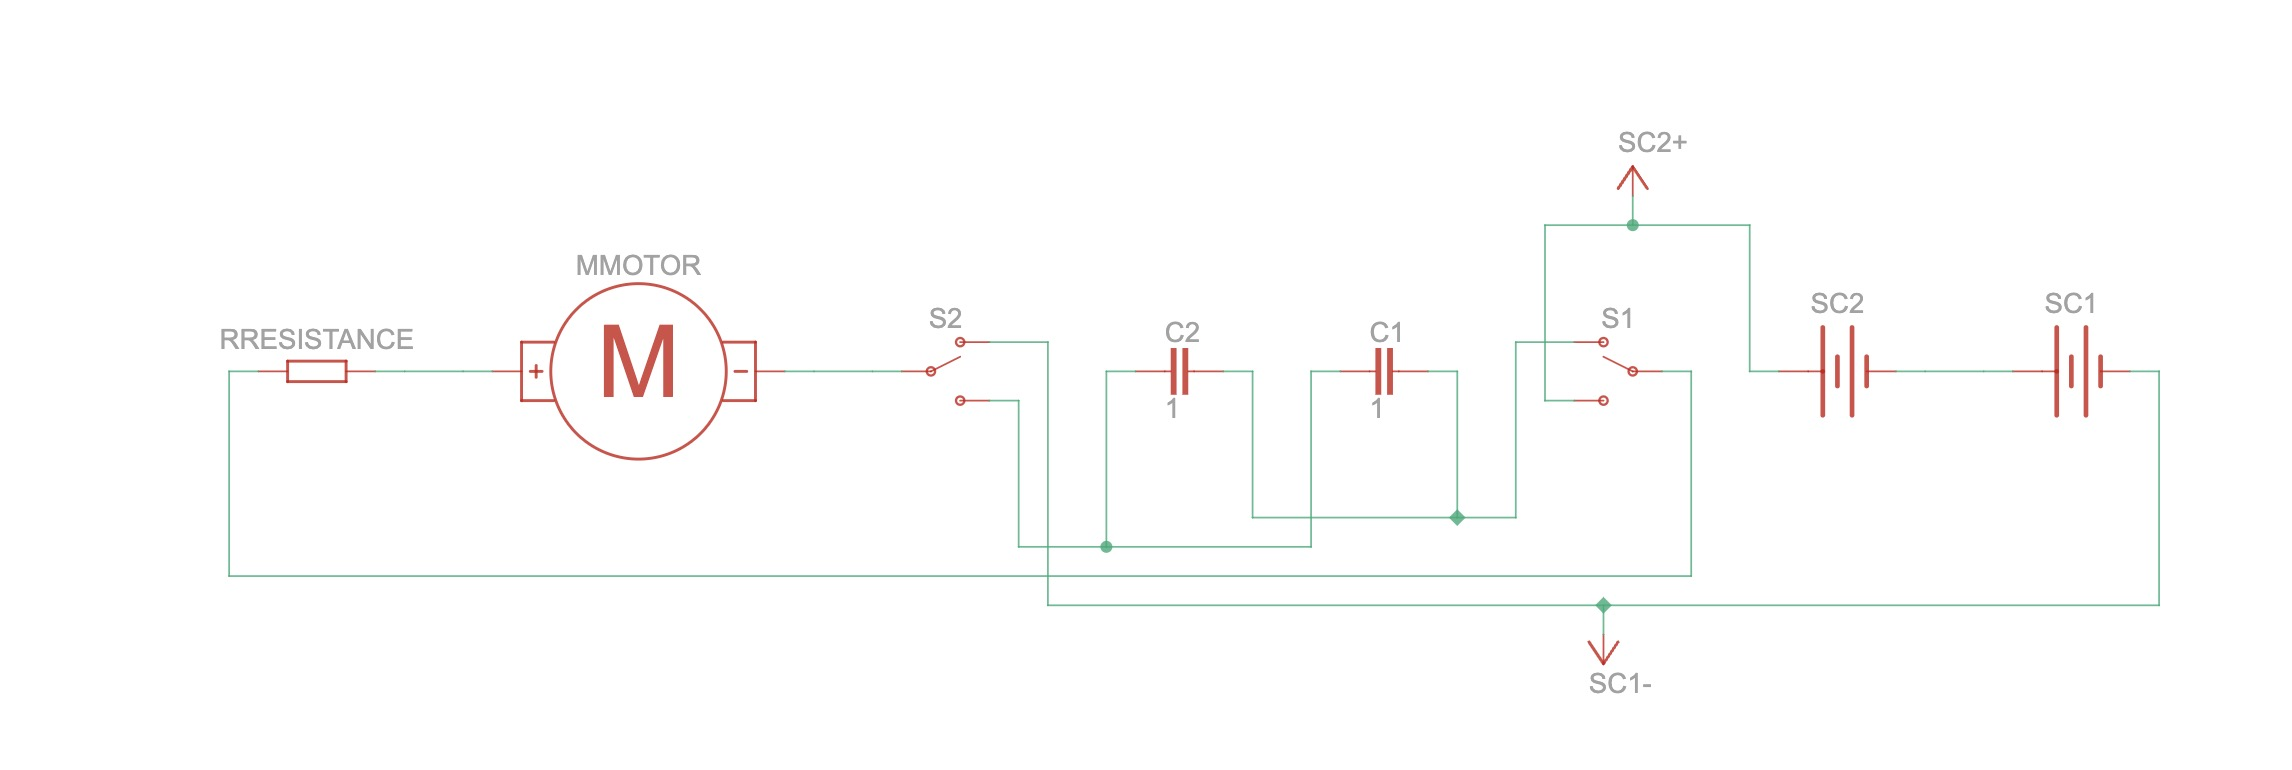
\includegraphics[width=1\textwidth]{figure/circute_design.jpeg} 
    \caption{Circuit Design} 
\end{figure}
\subsection{Material Selection}
After our group evaluation meeting, plastic and plywood were selected for their affordability and ease of processing.
Plastic allows for precision using 3D printing and CAD designs, 
while wood provides an affordable alternative for certain parts. 
Carbon fiber was excluded due to its high cost and processing fees.
\subsection{Transmission System}
By merging all the ideas and primary test, we have decided to use Gearbox as the transmission system.
Direct Drive was found inefficient due to motor limitations.
The Gearbox offers better power efficiency but is harder to design. 
Belt Drive is also effective but requires redesigning the entire power system, 
which complicates motor usage. Therefore, Gearbox will be the primary choice, with Belt Drive as a fallback if Gearbox fails.
Here is our gearbox and motor design.
\begin{figure}[h] 
    \centering 
    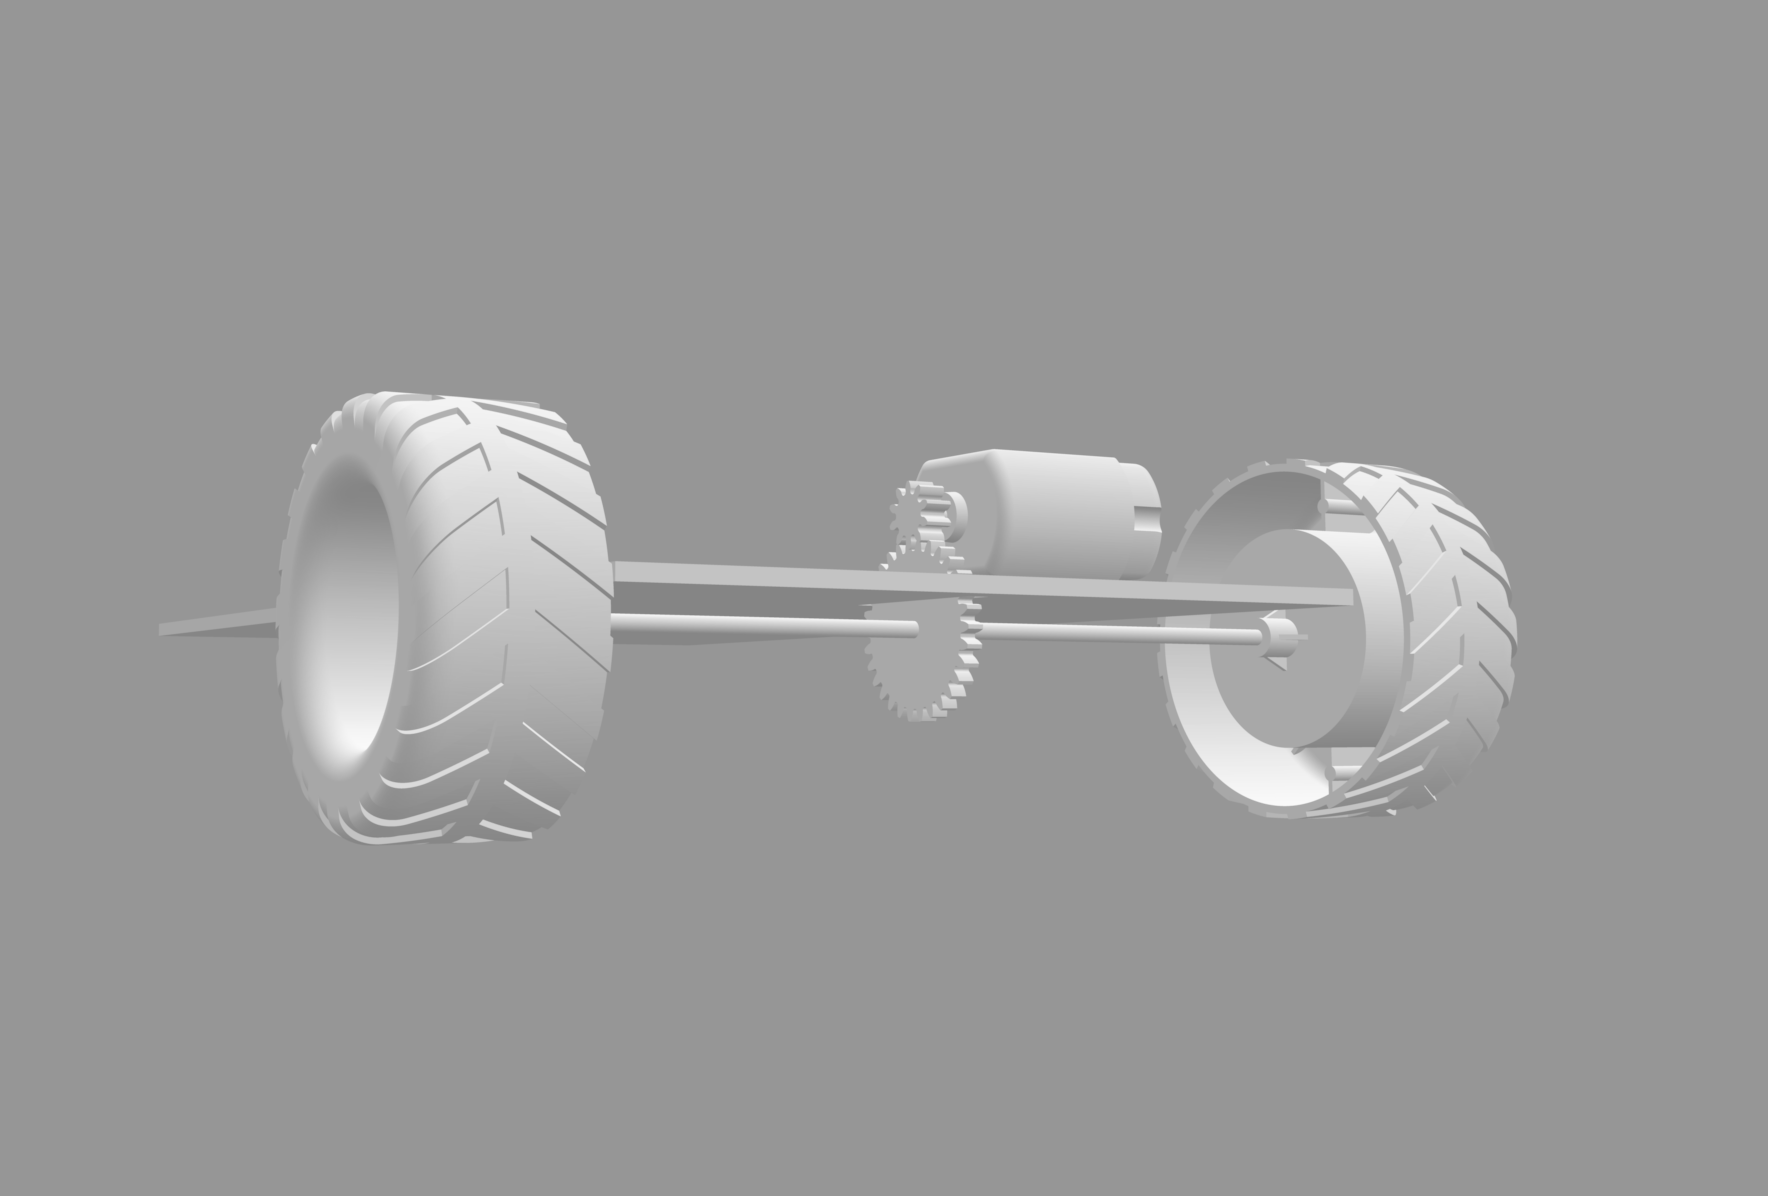
\includegraphics[width=1\textwidth]{figure/gearbox_design.png} 
    \caption{motor and gearbox design} 
\end{figure}
\subsection{Appearance}
After our group evaluation meeting, we have decided merge curved shape and box shape as the appearance of our solar-powered car.
The curved shape can reduce the air resistance and make the car more marketable. And at the middle of the car, we will use the box shape to make 
it eaiser to install the motor and gearbox. At the top, solar panel will be the roof of the car. Such design also make it lighter and faster.
Here is our appearance design.
\begin{figure}[h] 
    \centering 
    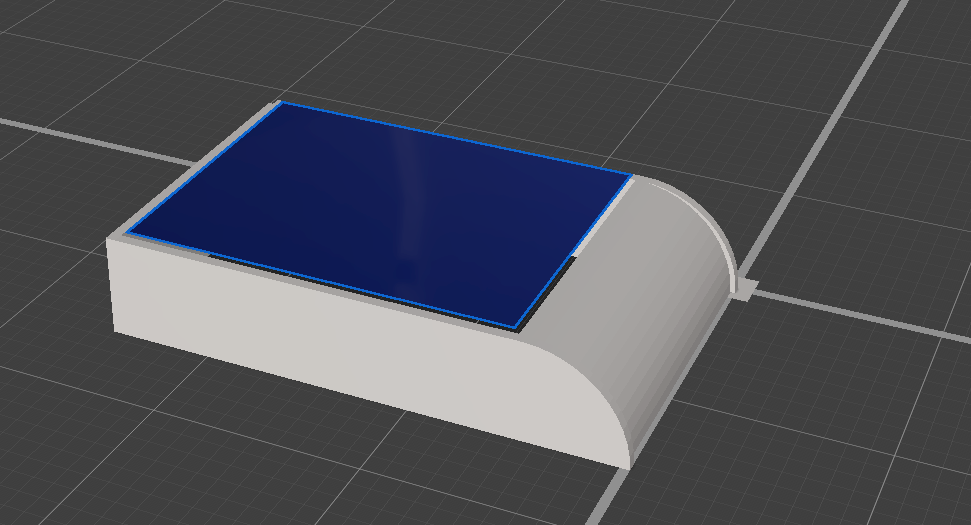
\includegraphics[width=1\textwidth]{figure/appearence.png} 
    \caption{motor and gearbox design} 
\end{figure}
\subsection{Solution overview}
Our solar car’s first version will have a plastic front-side, wood base and wood side. 
Both solar panels and capacitors will be integrated. 
Weight considerations will be secondary to getting the car running as quickly as possible. 
A single motor and Gearbox system will power the car.

\newpage
\section{Project Planning}

\subsection{Gantt Chart}
Here is the Gantt Chart of our project planning to help you understand our project planing better. 
\begin{figure}[h] 
    \centering 
    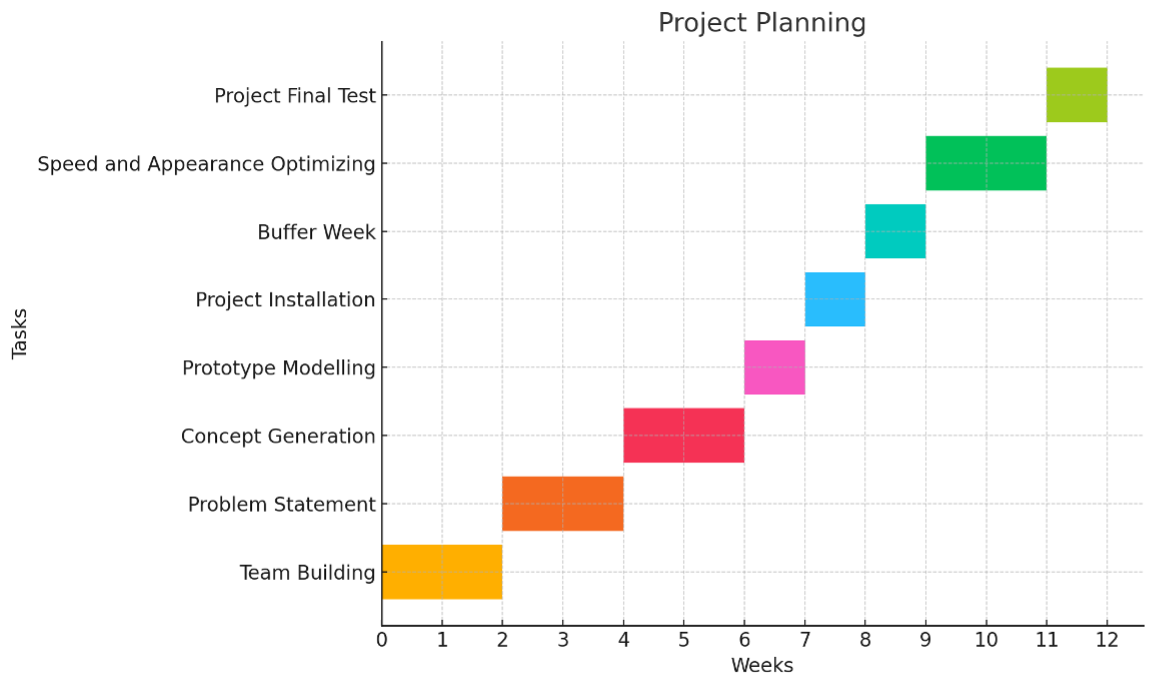
\includegraphics[width=0.8\textwidth]{figure/Picture1.png} 
    \caption{Gantt Chart} 
\end{figure}

\begin{table}[h!]
    \centering
    \begin{tabular}{|>{\raggedright\arraybackslash}p{3cm}|>{\raggedright\arraybackslash}p{4.5cm}|>{\raggedright\arraybackslash}p{6cm}|}
        \hline
        \textbf{Responsibility} & \textbf{Assigned Members} & \textbf{Description} \\ 
        \hline
        3D Printing Design Map & Chi-En Peng, Yung-Ching Liang & 
        Accelerates project development and helps achieve precise design outcomes. \\ 
        \hline
        Gearbox & Yaran Zhang, Shenglin Wang & 
        Contains gears, bearings, input shaft, output shaft, and housing. Provides torque amplification and load distribution. \\ 
        \hline
        Power System & Weijia Xiao & 
        Ensures continuous power supply from solar panels to power the car efficiently. \\ 
        \hline
        Organizing  \& Laser Cutting  & Cheong Zhang & 
        Organize the team and assign tasks \&Ensures accurate splicing of frames and reduces material waste. \\ 
        \hline
        Measurement & Yaran Zhang, Yixuan Wu, Chengrui Jiang & 
        Ensures components fit together correctly and machines operate efficiently through precise measurements. \\ 
        \hline
    \end{tabular}
    \caption{Roles and Responsibilities in Solar-Powered Car Project}
\end{table}
\subsection{Previous Work}
In the first six weeks, we completed three theoretical parts: Team Building, Problem Statement, and Concept Generation. In Week 1, team members got to know each other and held the first group meeting, where everyone presented their understanding of the problem statement. In Week 3, the problem statement facilitated more productive group discussions, as the outcomes were more comprehensive and feasible than individual solutions. By Week 5, the team delivered a presentation on concept generation, exploring various materials, power sources, and transmission methods to optimize performance by balancing efficiency, cost, and weight.
\subsection{prototype modeling}
Using a well-equipped car for simple tests was impractical, so we started with temporary substitutes. 
As shown in figure  ~\ref{pic:prototype_car}, the body and bottom plate were made of cardboard, with a motor, solar panels, and wheels installed. 
The car ran successfully, but its speed was unsatisfactory. 
Additional materials were acquired, and further testing will aim to reduce weight and improve speed.

\subsection{Project installation}
\label{sec:installation}
To install the car, we have decided the components that may be used in our solar panel car.
Such as the solar panel, DC Motor, wheels, base, the shell, gears, transmission shaft and some wires to transfer electric energy. 
Careful selection and placement of components, such as the solar panel, motor, wheels, and transmission system, is important to ensure a balanced and smooth-running car\cite{Hapuwatte2017}. 
\subsection{Speed and Appearance optimization}
\label{sec:Optimization}  
To achieve high speed, we focused on reducing weight and minimizing components. After building the first version, we removed or replaced parts to make it lighter and faster. 
Friction within the power system, including the gearbox and transmission shaft, was minimized. 
On cloudy days, capacitors will power the car, requiring resistor optimization. 
We will also test and adjust the gear ratio to maximize speed. Additionally, the car's appearance will be refined to enhance market appeal.

\subsection{Project Final Test}
In the final test, we aim to have a high speed within competitors. Under the full support of previous test and optimization, we believe our car will have a high speed.
\subsection{Risk Management}
The main risk are \textbf{shortage of makerspace resource(equipment and material), unexpected installation detail and weather condition during optimization}, which could delay the project.
\\
\\
To mitigate the first two risks, we will have a buffer week between the \textit{\hyperref[sec:installation]{Project Installation}} and \textit{\hyperref[sec:Optimization]{Speed and Appearance optimization}}. 
This week will be used to address the problems and unexpected detail that may occur in the "Project installation" part. This buffer week will provide extra time to resolve any unexpected detail that may occur during the installation period.
It ensures that out team have flexibility to address those issues without delaying the whole project.
\\
\\
Futhermore, the buffer week can also partially mitigate the risk caused by poor weather conditions during the testing and optimization phase. 
If we encounter days with poor weather that limit outdoor testing with solar panels, 
this extra time will allow us to shift tests around.
\\
\\
In addition to the buffer week, we will have a \textbf{backup plan} to reduce the impact of adverse weather. Specifically, during the testing and optimization period, 
we will simulate solar panel using batteries with adjustable voltage and current                                           . 
This approach will allow us to continue our optimization efforts without delay, 
even if real-time solar energy tests are limited by poor weather. 
This backup plan ensures that our progress remains steady and the project stays on track regardless of external environmental factors.

\subsection{Budget}
This is our current budget breakdown for the project, which includes the cost of almost all parts and materials needed to build the solar-powered car.

\begin{table}[h] 
\centering 
\begin{tabularx}{\textwidth}{Xrr}
\toprule
Parts & Total Qty & Total \$ \\
\midrule
wheels - 40mm & 4.0 & 1.40 \\
Motor F18 & 1.0 & 2.20 \\
Toggle switch two way blue & 1.0 & 3.00 \\
Pinion Gear 10Tooth & 2.0 & 0.60 \\
Pinion Gear 12Tooth & 2.0 & 0.60 \\
Spur Gear 36 Tooth & 5.0 & 2.75 \\
Spur Gear48Tooth & 4.0 & 2.20 \\
Spur Gear54Tooth & 4.0 & 2.20 \\
Spur Gear60Tooth & 3.0 & 1.65 \\
Spur Gear 48/12 Tooth & 1.0 & 0.60 \\
Motor Mount 3D printed - Basic & 1.0 & 1.00 \\
Motor Mount 3D printed - F13 \& F18 & 1.0 & 1.00 \\
Solar panel 2v & 2.0 & 17.00 \\
Corflute 400 x 400 & 1.0 & 4.00 \\
Capacitor & 2.0 & 7.30 \\
Axle Collar/bush & 5.0 & 0.70 \\
F/Glass Axle 3mm x 167mm long & 2.0 & 0.90 \\
Other - Double sided tape, glue, bolts and washers & 1.0 & 4.00 \\
\midrule
Total & 45.0 & 52.70 \\
\bottomrule
\end{tabularx}
\caption{Budget Breakdown for Parts}
\end{table}
\section{Conclusion}
(about half to one page)
Will be finished in Oct 14 night.

\newpage
\addcontentsline{toc}{section}{References}
\printbibliography

\newpage
\section{Appendix}
\pagenumbering{arabic}  
\setcounter{page}{1}
This appendix contains supplementary materials such as detailed calculations, additional diagrams, or extended descriptions related to the project.
\begin{figure}[h] 
    \centering 
    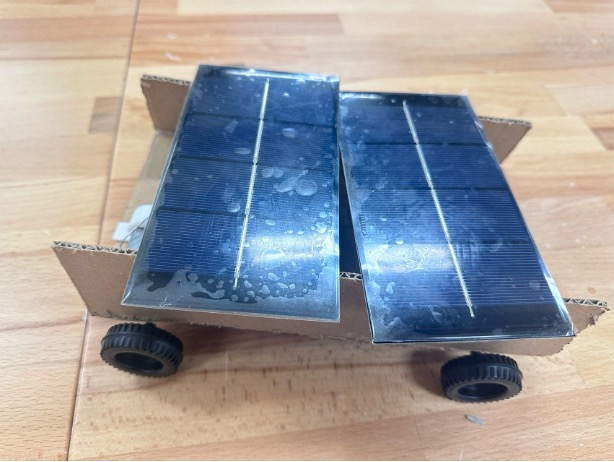
\includegraphics[width=0.8\textwidth]{figure/car_prototype.jpg} 
    \caption{Prototype Car}
    \label{pic:prototype_car}
\end{figure}
\begin{figure}[h] 
    \centering 
    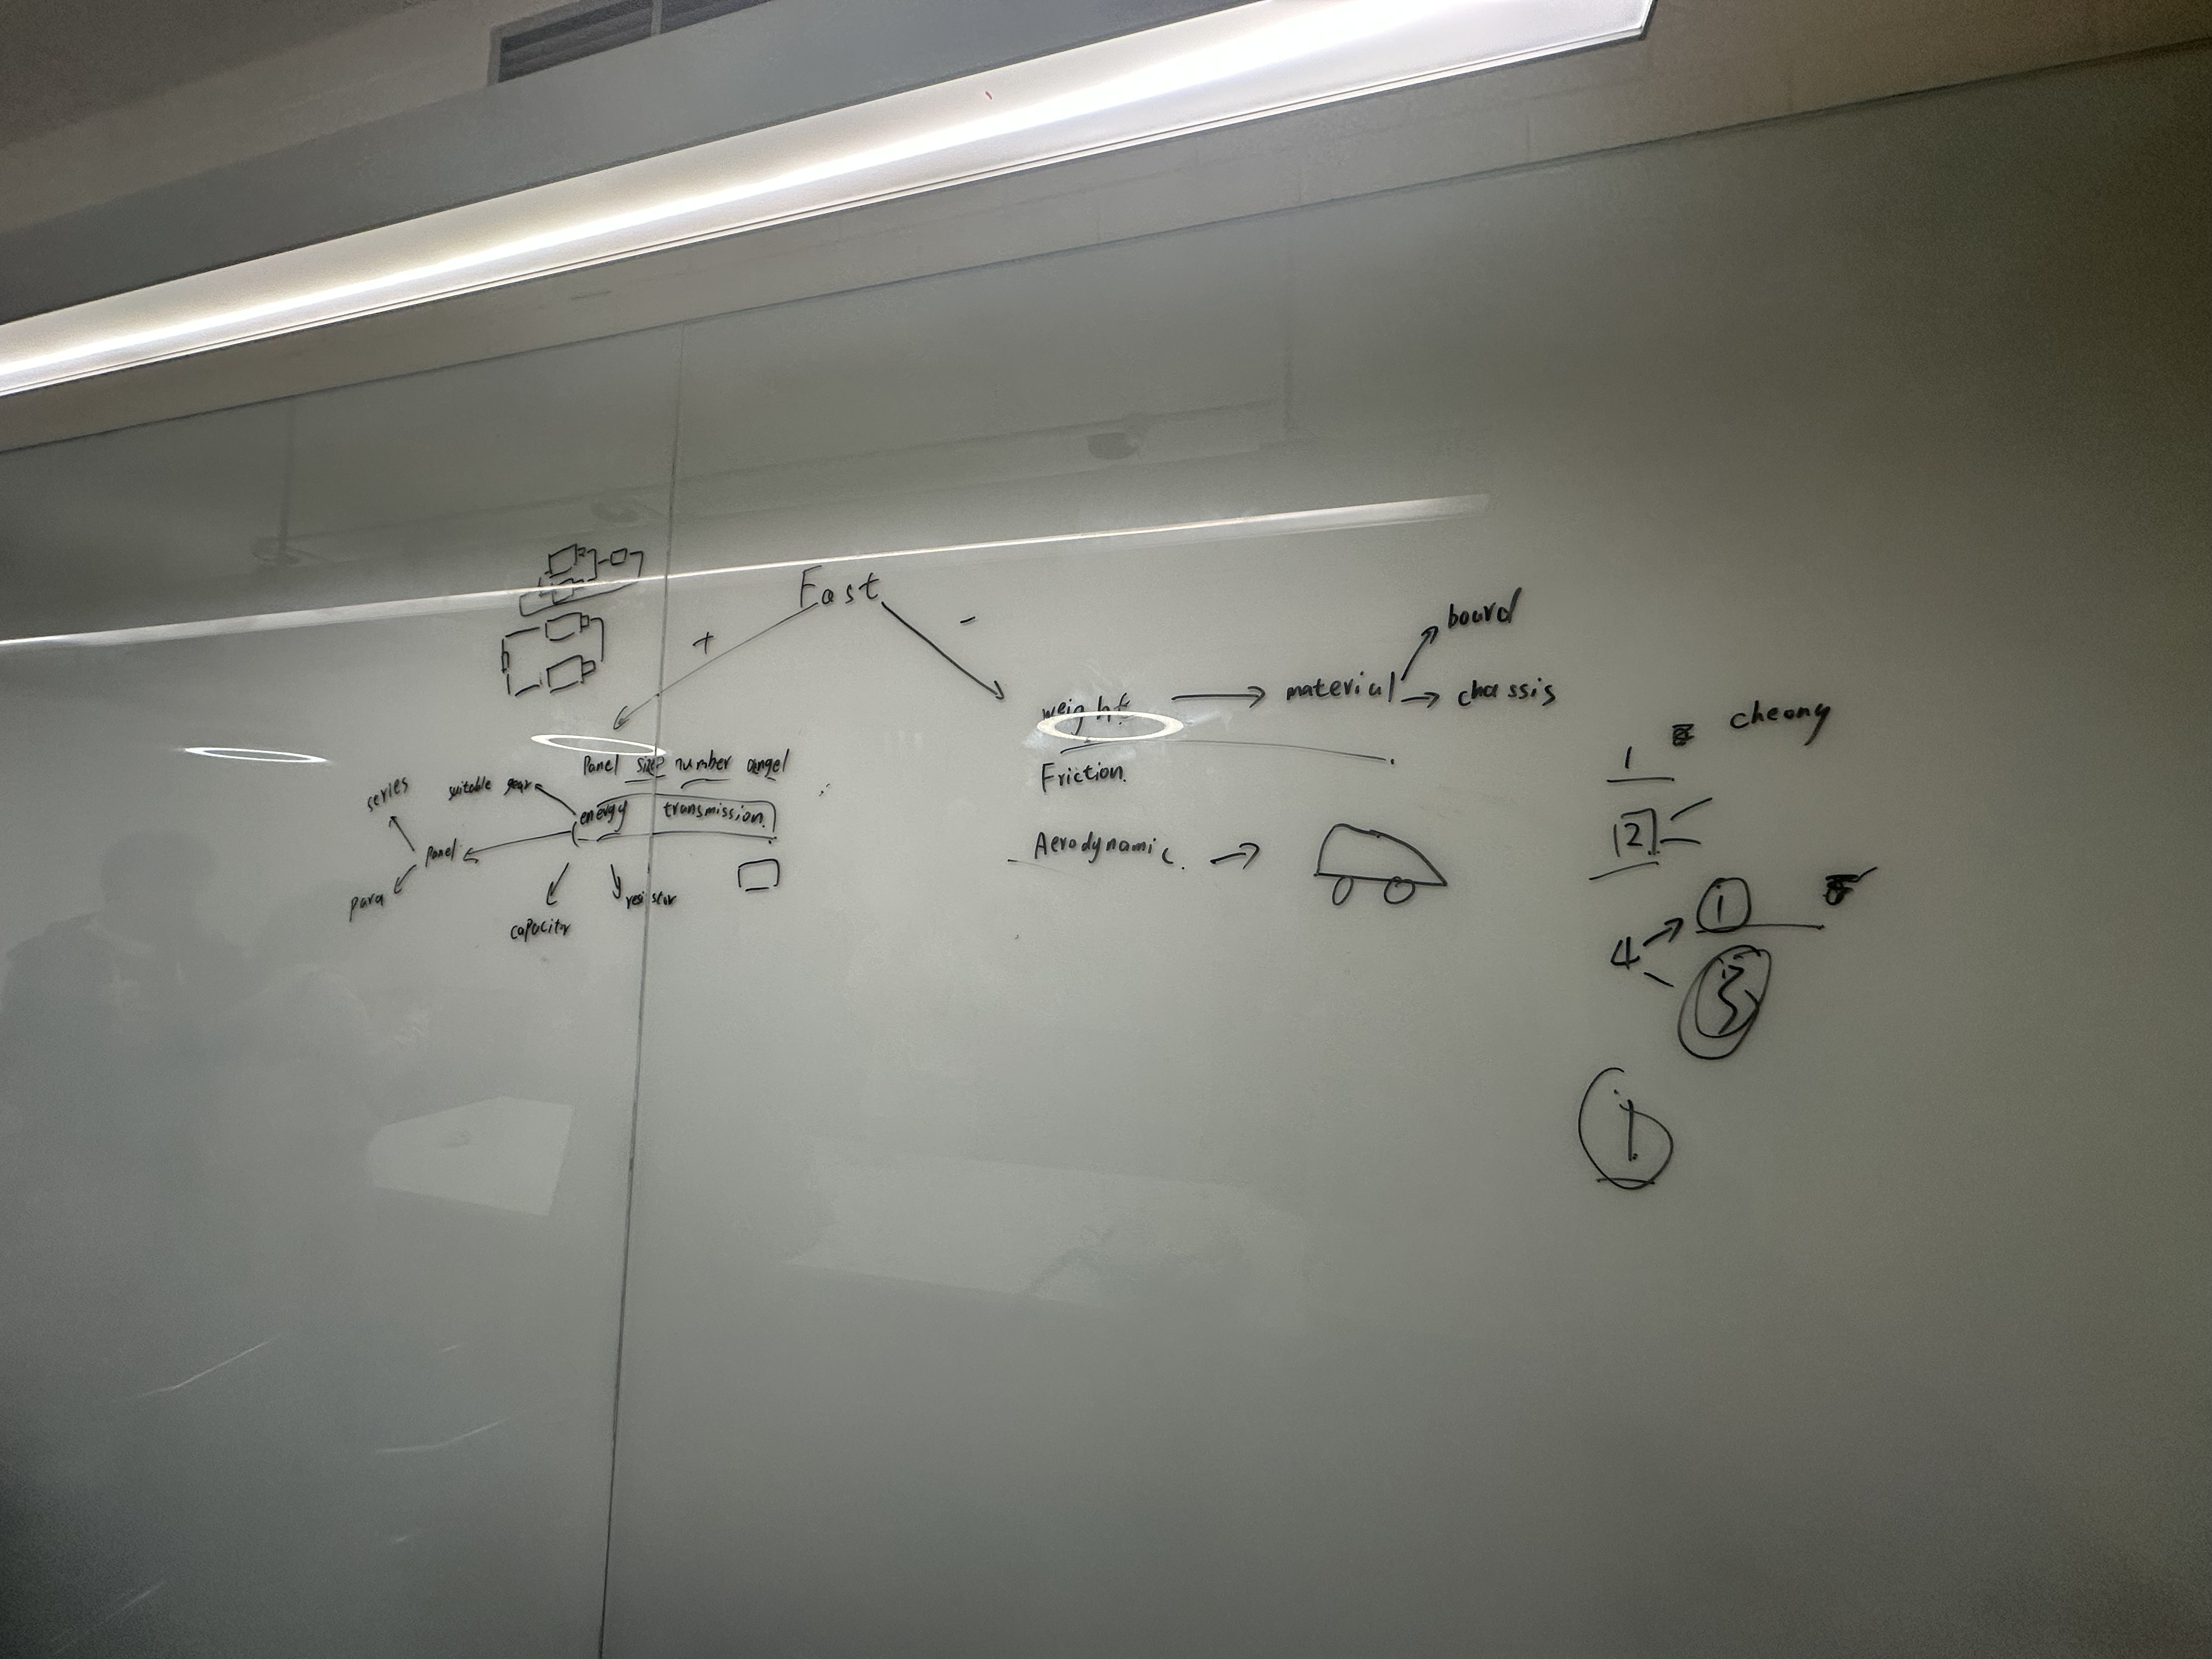
\includegraphics[width=0.8\textwidth]{figure/function_tree.jpg} 
    \caption{Function tree}
    \label{pic:function tree}
\end{figure}
\end{document}



